\documentclass[conference]{IEEEtran}

% ── Paquetes ──────────────────────────────────────────────────────
\usepackage[utf8]{inputenc}
\usepackage[spanish,es-nodecimaldot]{babel}
\usepackage{graphicx}
\usepackage{amsmath,amssymb}
\usepackage{booktabs}
\usepackage{tabularx}
\usepackage{multirow}
\usepackage[hidelinks]{hyperref}
\usepackage{float}
\usepackage{subcaption}
\usepackage{xcolor}
\usepackage{listings}
\usepackage{cite}
\usepackage{url}

% ── Rutas de figuras ──────────────────────────────────────────────
\graphicspath{{../../outputs/figures/}}

% ── Metadatos ─────────────────────────────────────────────────────
\title{Clasificación de Tumores Cerebrales en MRI mediante
Redes Neuronales Convolucionales propias sobre el Dataset
\textit{Brain Tumor Classification MRI}}

\author{\IEEEauthorblockN{Abel Albuez Sánchez, Daniel Rios,
Juan Torres y Javier Esquivel%
\thanks{Repositorio del proyecto: \url{https://github.com/AbelAlbuez/deep-learning-class/tree/main/proyecto-final}}}
\IEEEauthorblockA{Maestría en Analítica para Inteligencia de
Negocios (MAIN)\\
Pontificia Universidad Javeriana, Bogotá D.C., Colombia\\
Profesor: Julio Omar Palacio Niño, M.Sc. \quad
Aprendizaje Profundo \quad 2026}}

\begin{document}

\maketitle

% ── Abstract ──────────────────────────────────────────────────────
\begin{abstract}
La clasificación automática de tumores cerebrales en imágenes
de resonancia magnética (MRI) constituye una tarea relevante
para el apoyo al diagnóstico radiológico. Este trabajo aborda
la clasificación de cuatro categorías ---\textit{glioma},
\textit{meningioma}, \textit{pituitary} y \textit{no tumor}---
sobre el dataset público \textit{Brain Tumor Classification MRI}
de Kaggle (3\,264 imágenes), mediante tres arquitecturas
propias de redes neuronales convolucionales (CNN) entrenadas
desde cero, sin emplear \textit{transfer learning}. Se reporta
un análisis exploratorio detallado del dataset
---incluyendo distribución por clases, dimensionalidad y
estadísticos de intensidad---, un pipeline de preprocesamiento
con normalización tipo ImageNet y \textit{data augmentation},
y un protocolo de evaluación basado en \textit{F1-Score} macro,
adecuado para escenarios con desbalance de clases.
\end{abstract}

\begin{IEEEkeywords}
clasificación de tumores cerebrales, redes neuronales
convolucionales, resonancia magnética, aprendizaje profundo,
PyTorch, F1-Score macro
\end{IEEEkeywords}

% ── Secciones ─────────────────────────────────────────────────────
\section{Objetivo del Proyecto}

\subsection{Contexto Clínico}
El diagnóstico temprano y preciso de tumores cerebrales constituye
uno de los retos más relevantes de la neuro-oncología
contemporánea. La resonancia magnética (MRI, \textit{Magnetic
Resonance Imaging}) es la modalidad de imagen de referencia para
la detección y caracterización de estas lesiones; sin embargo, su
interpretación depende fuertemente de la experiencia del radiólogo
y está sujeta a variabilidad inter-observador. En este contexto,
los sistemas de apoyo al diagnóstico basados en aprendizaje
profundo han mostrado resultados prometedores como herramientas
de cribado y segunda opinión, capaces de procesar grandes
volúmenes de estudios de manera consistente.

\subsection{Objetivo Técnico}
El presente proyecto tiene como objetivo diseñar, entrenar y
evaluar tres arquitecturas propias de redes neuronales
convolucionales (CNN) para la clasificación automática de
imágenes MRI cerebrales en cuatro categorías:
\textit{glioma\_tumor}, \textit{meningioma\_tumor},
\textit{no\_tumor} y \textit{pituitary\_tumor}. Se utiliza el
dataset público \textit{Brain Tumor Classification MRI} disponible
en Kaggle. De manera explícita, este trabajo \textbf{no} emplea
técnicas de \textit{transfer learning} ni pesos preentrenados
sobre ImageNet u otros corpus; el énfasis pedagógico está en la
construcción de arquitecturas convolucionales desde cero y en la
comprensión del impacto de sus hiperparámetros y bloques
constitutivos.

\subsection{Criterios de Evaluación}
La evaluación de los modelos se realizará mediante un conjunto
de métricas clásicas de clasificación multiclase:
\textit{Accuracy}, \textit{Precision}, \textit{Recall} y
\textit{F1-Score} en su variante \textit{macro-averaged},
complementadas con la matriz de confusión por modelo. Dado el
desbalance entre clases observado durante el análisis exploratorio
(Sección~\ref{sec:eda}), el \textit{F1-macro} se adopta como
métrica principal de comparación, por su robustez frente a clases
minoritarias.

\section{Análisis del Dataset y Dimensionalidad}
\label{sec:eda}

\subsection{Descripción del Dataset}
El conjunto de datos \textit{Brain Tumor Classification MRI},
publicado en Kaggle, contiene \textbf{3\,264 imágenes} de
resonancia magnética cerebral organizadas en cuatro clases
diagnósticas: \textit{glioma\_tumor}, \textit{meningioma\_tumor},
\textit{pituitary\_tumor} y \textit{no\_tumor} (estudios sin
hallazgos tumorales). Los autores del dataset proporcionan una
partición oficial entre conjuntos de entrenamiento y prueba que
se respeta en este trabajo. La Tabla~\ref{tab:dist} resume su
distribución.

\begin{table}[!t]
\centering
\caption{Distribución de imágenes por clase y partición.}
\label{tab:dist}
\begin{tabular}{lrrr}
\toprule
\textbf{Clase} & \textbf{Train} & \textbf{Test} & \textbf{Total} \\
\midrule
glioma\_tumor      & 826 & 100 & 926 \\
meningioma\_tumor  & 822 & 115 & 937 \\
no\_tumor          & 395 & 105 & 500 \\
pituitary\_tumor   & 827 &  74 & 901 \\
\midrule
\textbf{Total}     & \textbf{2\,870} & \textbf{394} & \textbf{3\,264} \\
\bottomrule
\end{tabular}
\end{table}

El conjunto de entrenamiento concentra el \textbf{87{,}9\,\%}
de las imágenes (2\,870), mientras que el conjunto de prueba
representa el \textbf{12{,}1\,\%} restante (394 imágenes). El
conjunto \textit{Testing} se reserva como \textit{holdout}
independiente para la evaluación final de los modelos, y la
subdivisión interna para validación se realiza únicamente sobre
\textit{Training} (véase Sección~\ref{sec:proto}).

\subsection{Balance de Clases}
El análisis de balance evidencia que la clase \textit{no\_tumor}
es la minoritaria en entrenamiento, con aproximadamente
\textbf{395} imágenes, frente a $\sim$\textbf{825} para cada una
de las tres clases tumorales. Esta proporción asimétrica
($\sim$1:2) puede inducir sesgos durante el aprendizaje, llevando
al modelo a sub-representar la clase minoritaria y a inflar
artificialmente la \textit{Accuracy} global.

Como estrategia de compensación se adopta el uso de pesos por
clase (\textit{class\_weight}) en la función de pérdida
\textit{Cross-Entropy}, con ponderaciones inversamente
proporcionales a la frecuencia relativa de cada clase en el
conjunto de entrenamiento. Esto incrementa la magnitud del
gradiente para errores cometidos sobre la clase minoritaria sin
alterar la distribución de muestras observadas. Las
Figuras~\ref{fig:balance} y \ref{fig:pie} ilustran gráficamente
esta distribución.

\begin{figure}[!t]
\centering
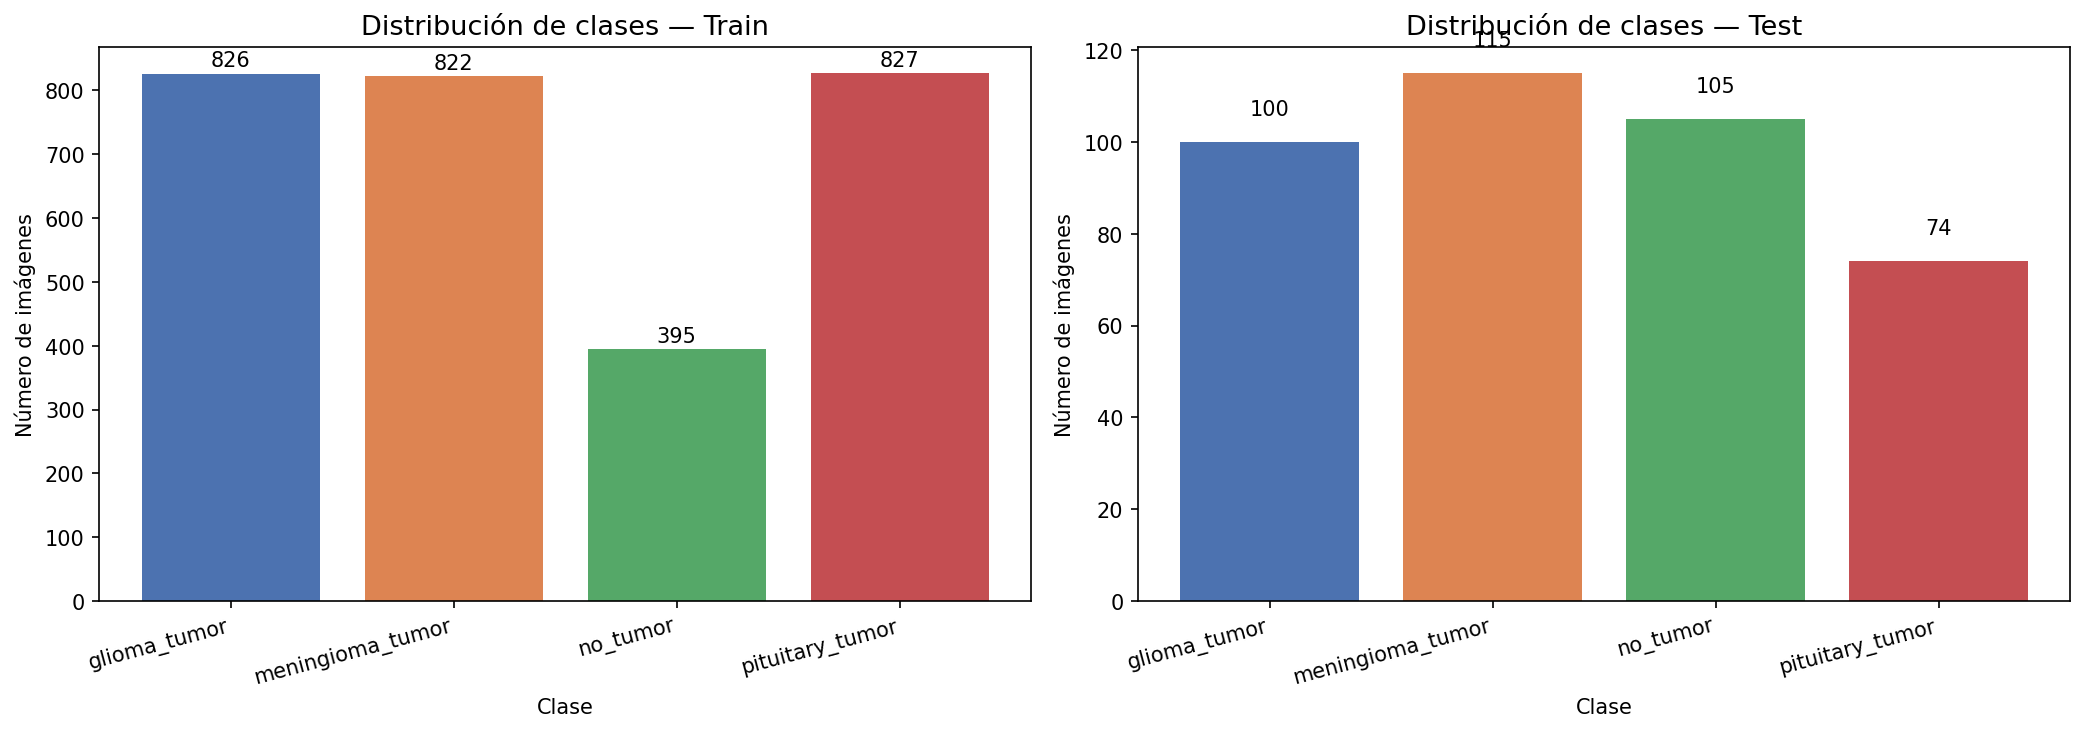
\includegraphics[width=\columnwidth]{../../outputs/figures/balance_clases.png}
\caption{Distribución absoluta por clase y partición.}
\label{fig:balance}
\end{figure}

\begin{figure}[!t]
\centering
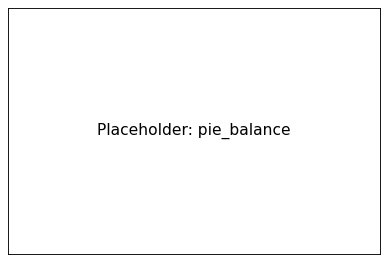
\includegraphics[width=0.75\columnwidth]{../../outputs/figures/pie_balance.png}
\caption{Proporción relativa en entrenamiento.}
\label{fig:pie}
\end{figure}

\subsection{Análisis de Dimensionalidad}
Se inspeccionó una muestra de \textbf{80 imágenes por clase}
para caracterizar la variabilidad en resolución espacial del
dataset. Las imágenes presentan resoluciones altamente
heterogéneas: las dimensiones máximas observadas alcanzan
\textbf{1024$\times$768\,px} y las mínimas \textbf{59$\times$80\,px}.
La relación de aspecto también varía considerablemente entre
estudios, reflejo de las diferencias entre equipos de adquisición
y protocolos clínicos.

Dada esta heterogeneidad, se establece el redimensionamiento
uniforme a \textbf{224$\times$224\,px} como paso obligatorio del
pipeline. Esta resolución constituye un compromiso adecuado
entre el nivel de detalle anatómico preservado y el costo
computacional, y es además el formato canónico de las
arquitecturas CNN modernas, lo que facilita comparaciones
posteriores. Las Figuras~\ref{fig:hist-res} y \ref{fig:aspect}
muestran respectivamente el histograma de resoluciones y la
distribución de relaciones de aspecto observadas por clase.

\begin{figure}[!t]
\centering
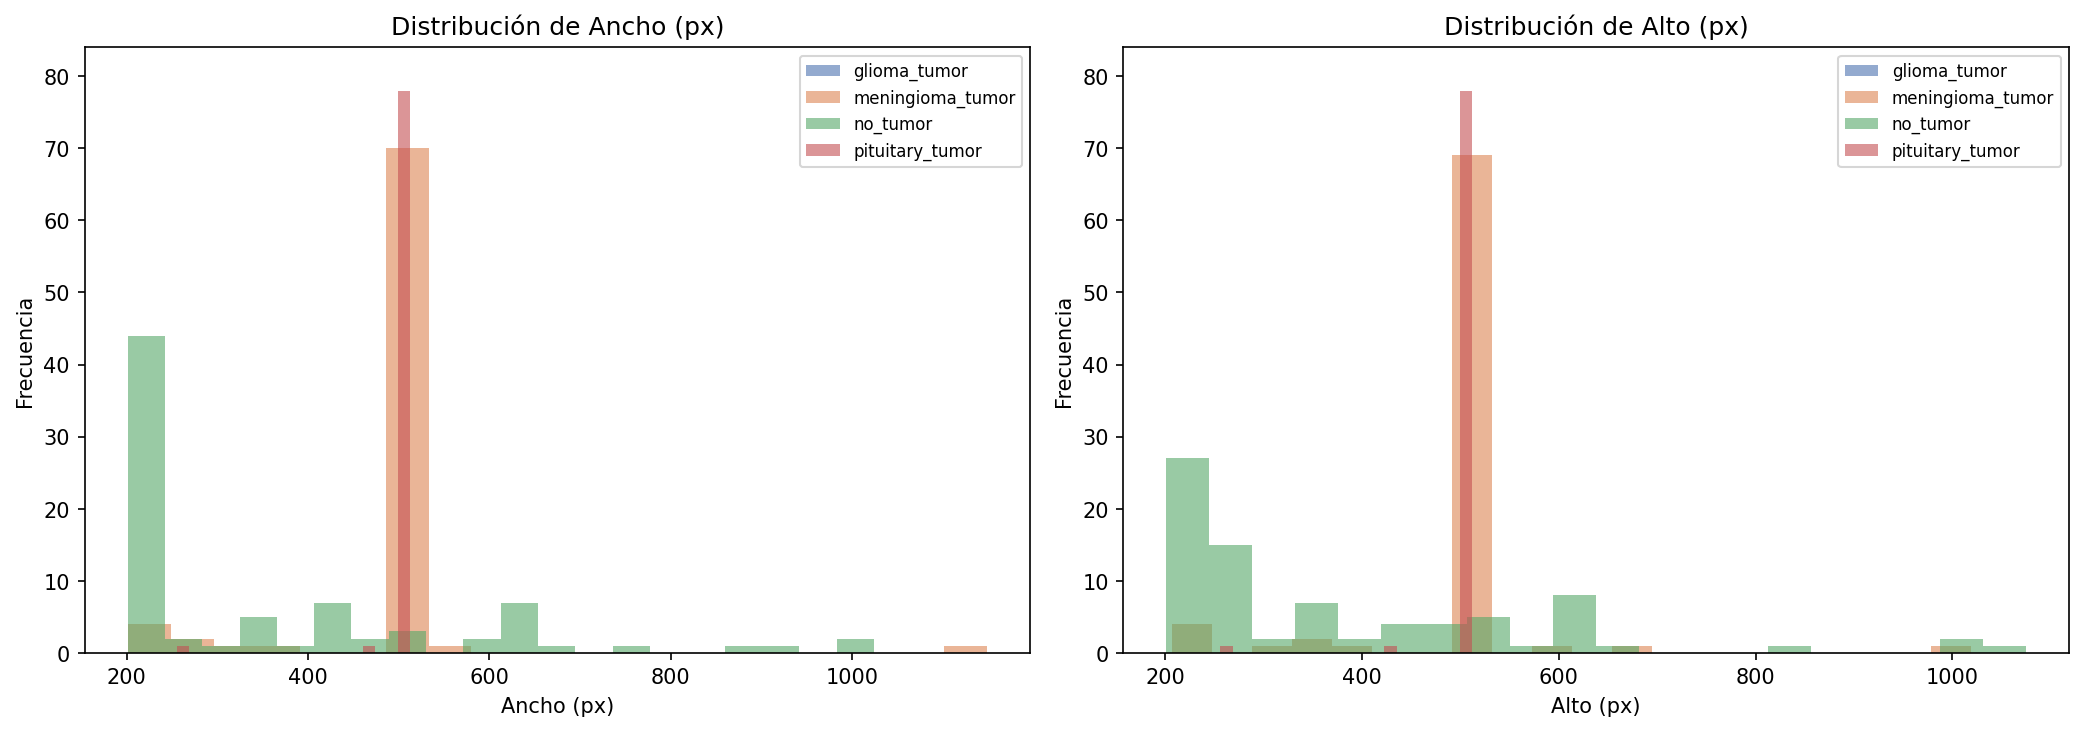
\includegraphics[width=\columnwidth]{../../outputs/figures/histograma_resolucion.png}
\caption{Histograma de resoluciones (ancho $\times$ alto) en el
dataset.}
\label{fig:hist-res}
\end{figure}

\begin{figure}[!t]
\centering
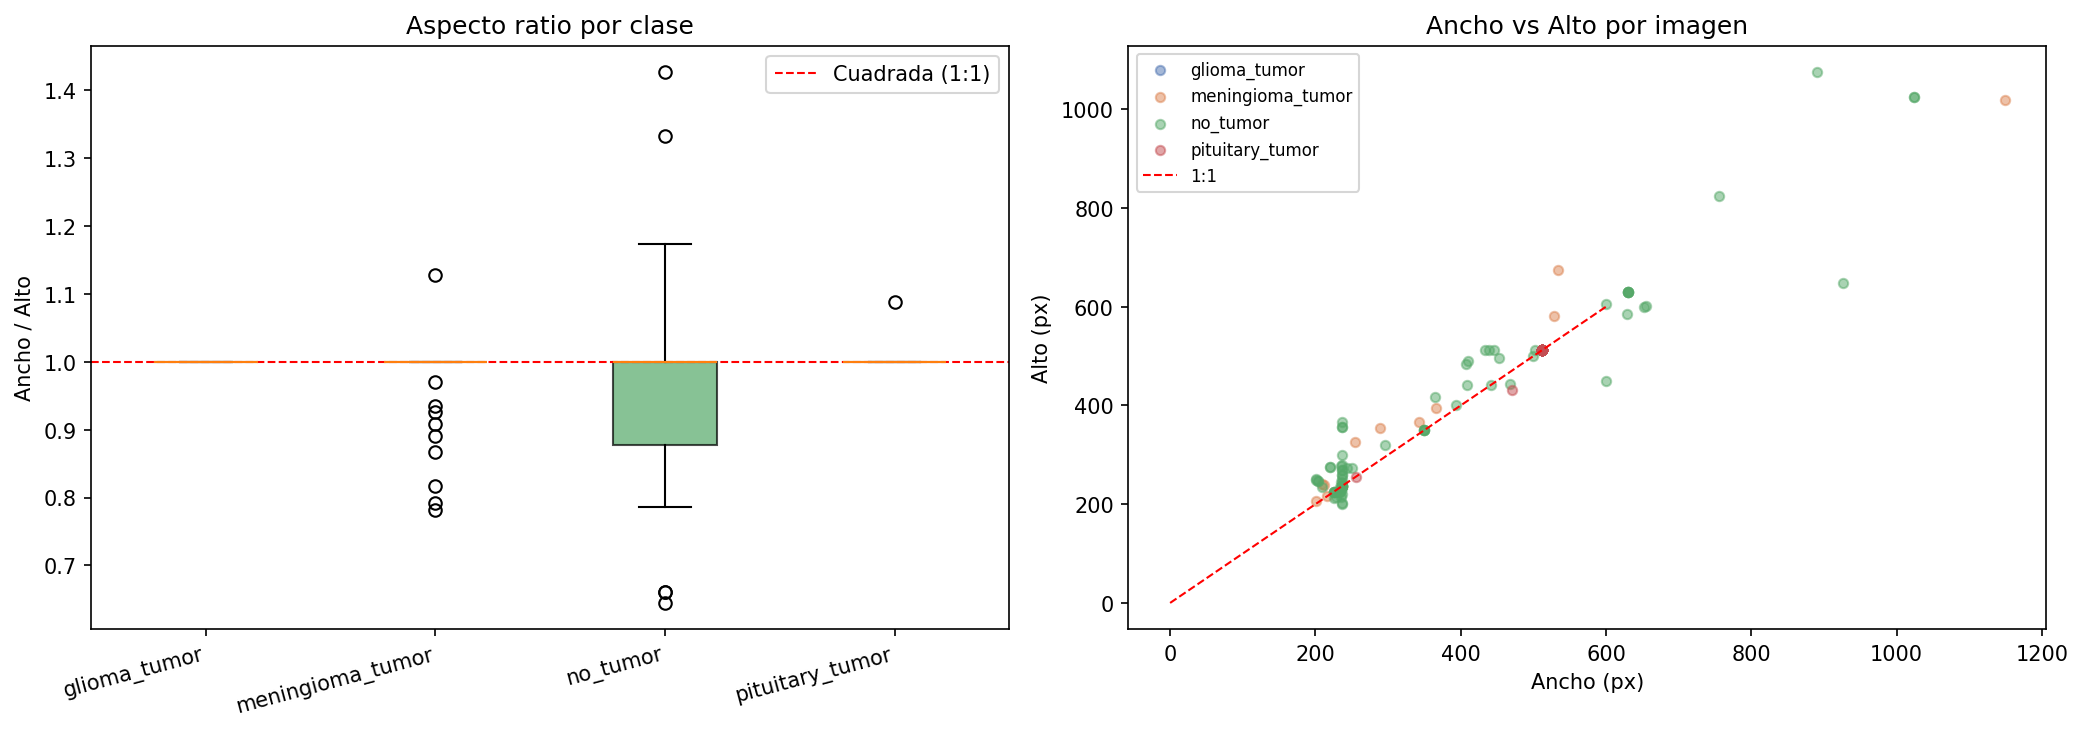
\includegraphics[width=\columnwidth]{../../outputs/figures/aspecto_ratio.png}
\caption{Distribución de relaciones de aspecto por clase.}
\label{fig:aspect}
\end{figure}

\subsection{Análisis Estadístico de Intensidades}
Se analizaron las distribuciones de intensidad de píxeles
(escala de grises) y canales RGB por clase, con el fin de
identificar diferencias fotométricas potencialmente
discriminativas para el modelado. La Tabla~\ref{tab:stats}
resume los estadísticos descriptivos.

\begin{table}[!t]
\centering
\caption{Estadísticas de intensidad (escala 0--255) por clase.}
\label{tab:stats}
\begin{tabular}{lrrrrr}
\toprule
\textbf{Clase} & \textbf{Media} & \textbf{Std} & \textbf{Mín} & \textbf{Máx} & \textbf{Mediana} \\
\midrule
glioma\_tumor     & 36{,}23 & 41{,}43 & 0 & 255 & 14 \\
meningioma\_tumor & 44{,}56 & 47{,}77 & 0 & 255 & 28 \\
no\_tumor         & 52{,}21 & 59{,}63 & 0 & 255 & 22 \\
pituitary\_tumor  & 49{,}50 & 42{,}94 & 0 & 255 & 50 \\
\bottomrule
\end{tabular}
\end{table}

Los \textit{gliomas} presentan los valores más bajos de media
(36{,}23) y mediana (14), lo que los caracteriza como tejidos
relativamente \textbf{hipointensos} en la modalidad analizada.
Los tumores \textit{pituitarios}, en contraste, presentan la
mediana más alta (50) y la menor dispersión relativa, indicando
intensidades más concentradas y homogéneas. La clase
\textit{no\_tumor} muestra la mayor desviación estándar
(59{,}63), consistente con la variedad anatómica del cerebro
sano sin focalización lesional. Estas diferencias fotométricas
constituyen señales útiles que una CNN puede explotar a nivel
de filtros convolucionales de bajo nivel.

Para estabilizar el entrenamiento se aplicará normalización
\textit{Z-score} sobre los tres canales utilizando los
estadísticos canónicos de ImageNet ($\mu = [0{,}485, 0{,}456,
0{,}406]$, $\sigma = [0{,}229, 0{,}224, 0{,}225]$), valores
ampliamente adoptados en la literatura como referencia robusta
incluso cuando no se emplea \textit{transfer learning}. Las
Figuras~\ref{fig:box} y \ref{fig:rgb} complementan visualmente
este análisis.

\begin{figure}[!t]
\centering
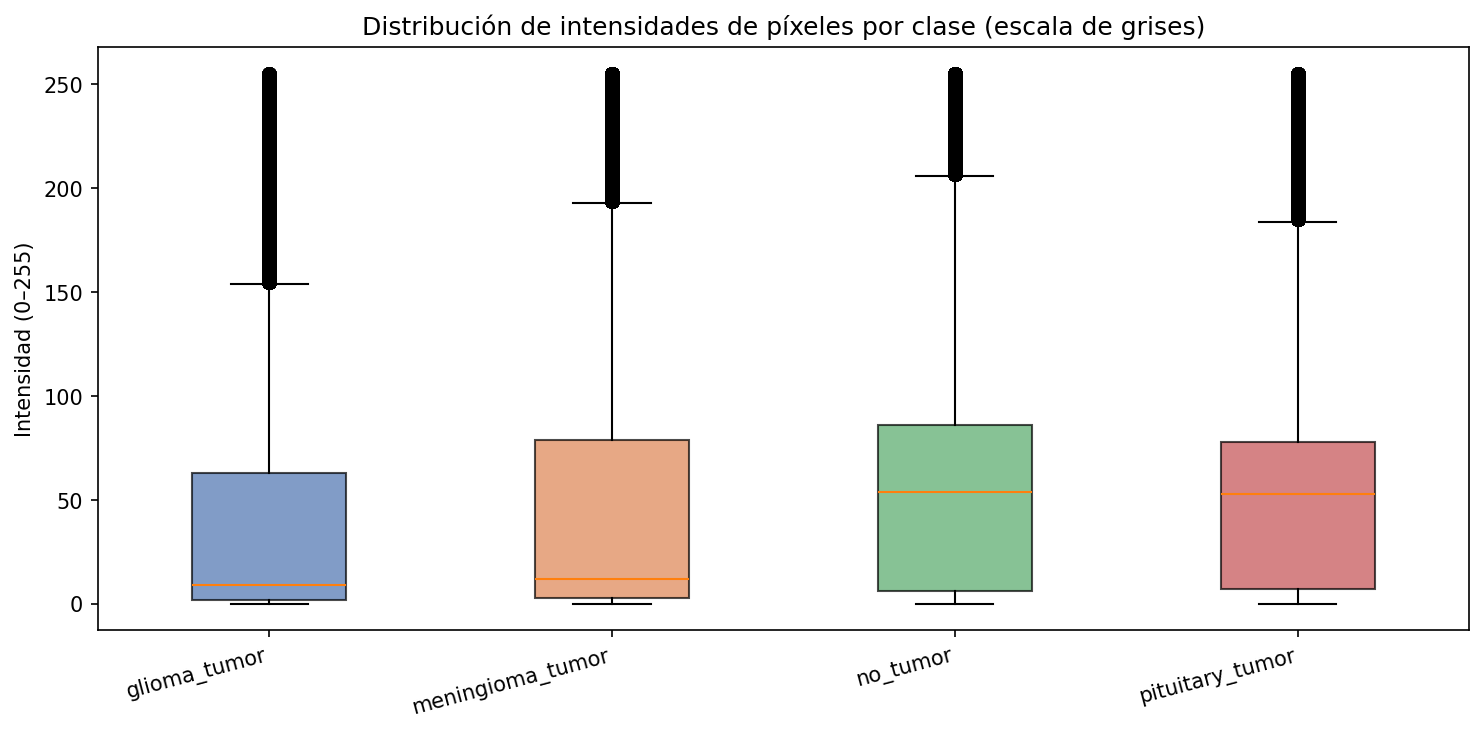
\includegraphics[width=\columnwidth]{../../outputs/figures/boxplot_intensidades.png}
\caption{Diagramas de caja de intensidades de píxel por clase.}
\label{fig:box}
\end{figure}

\begin{figure}[!t]
\centering
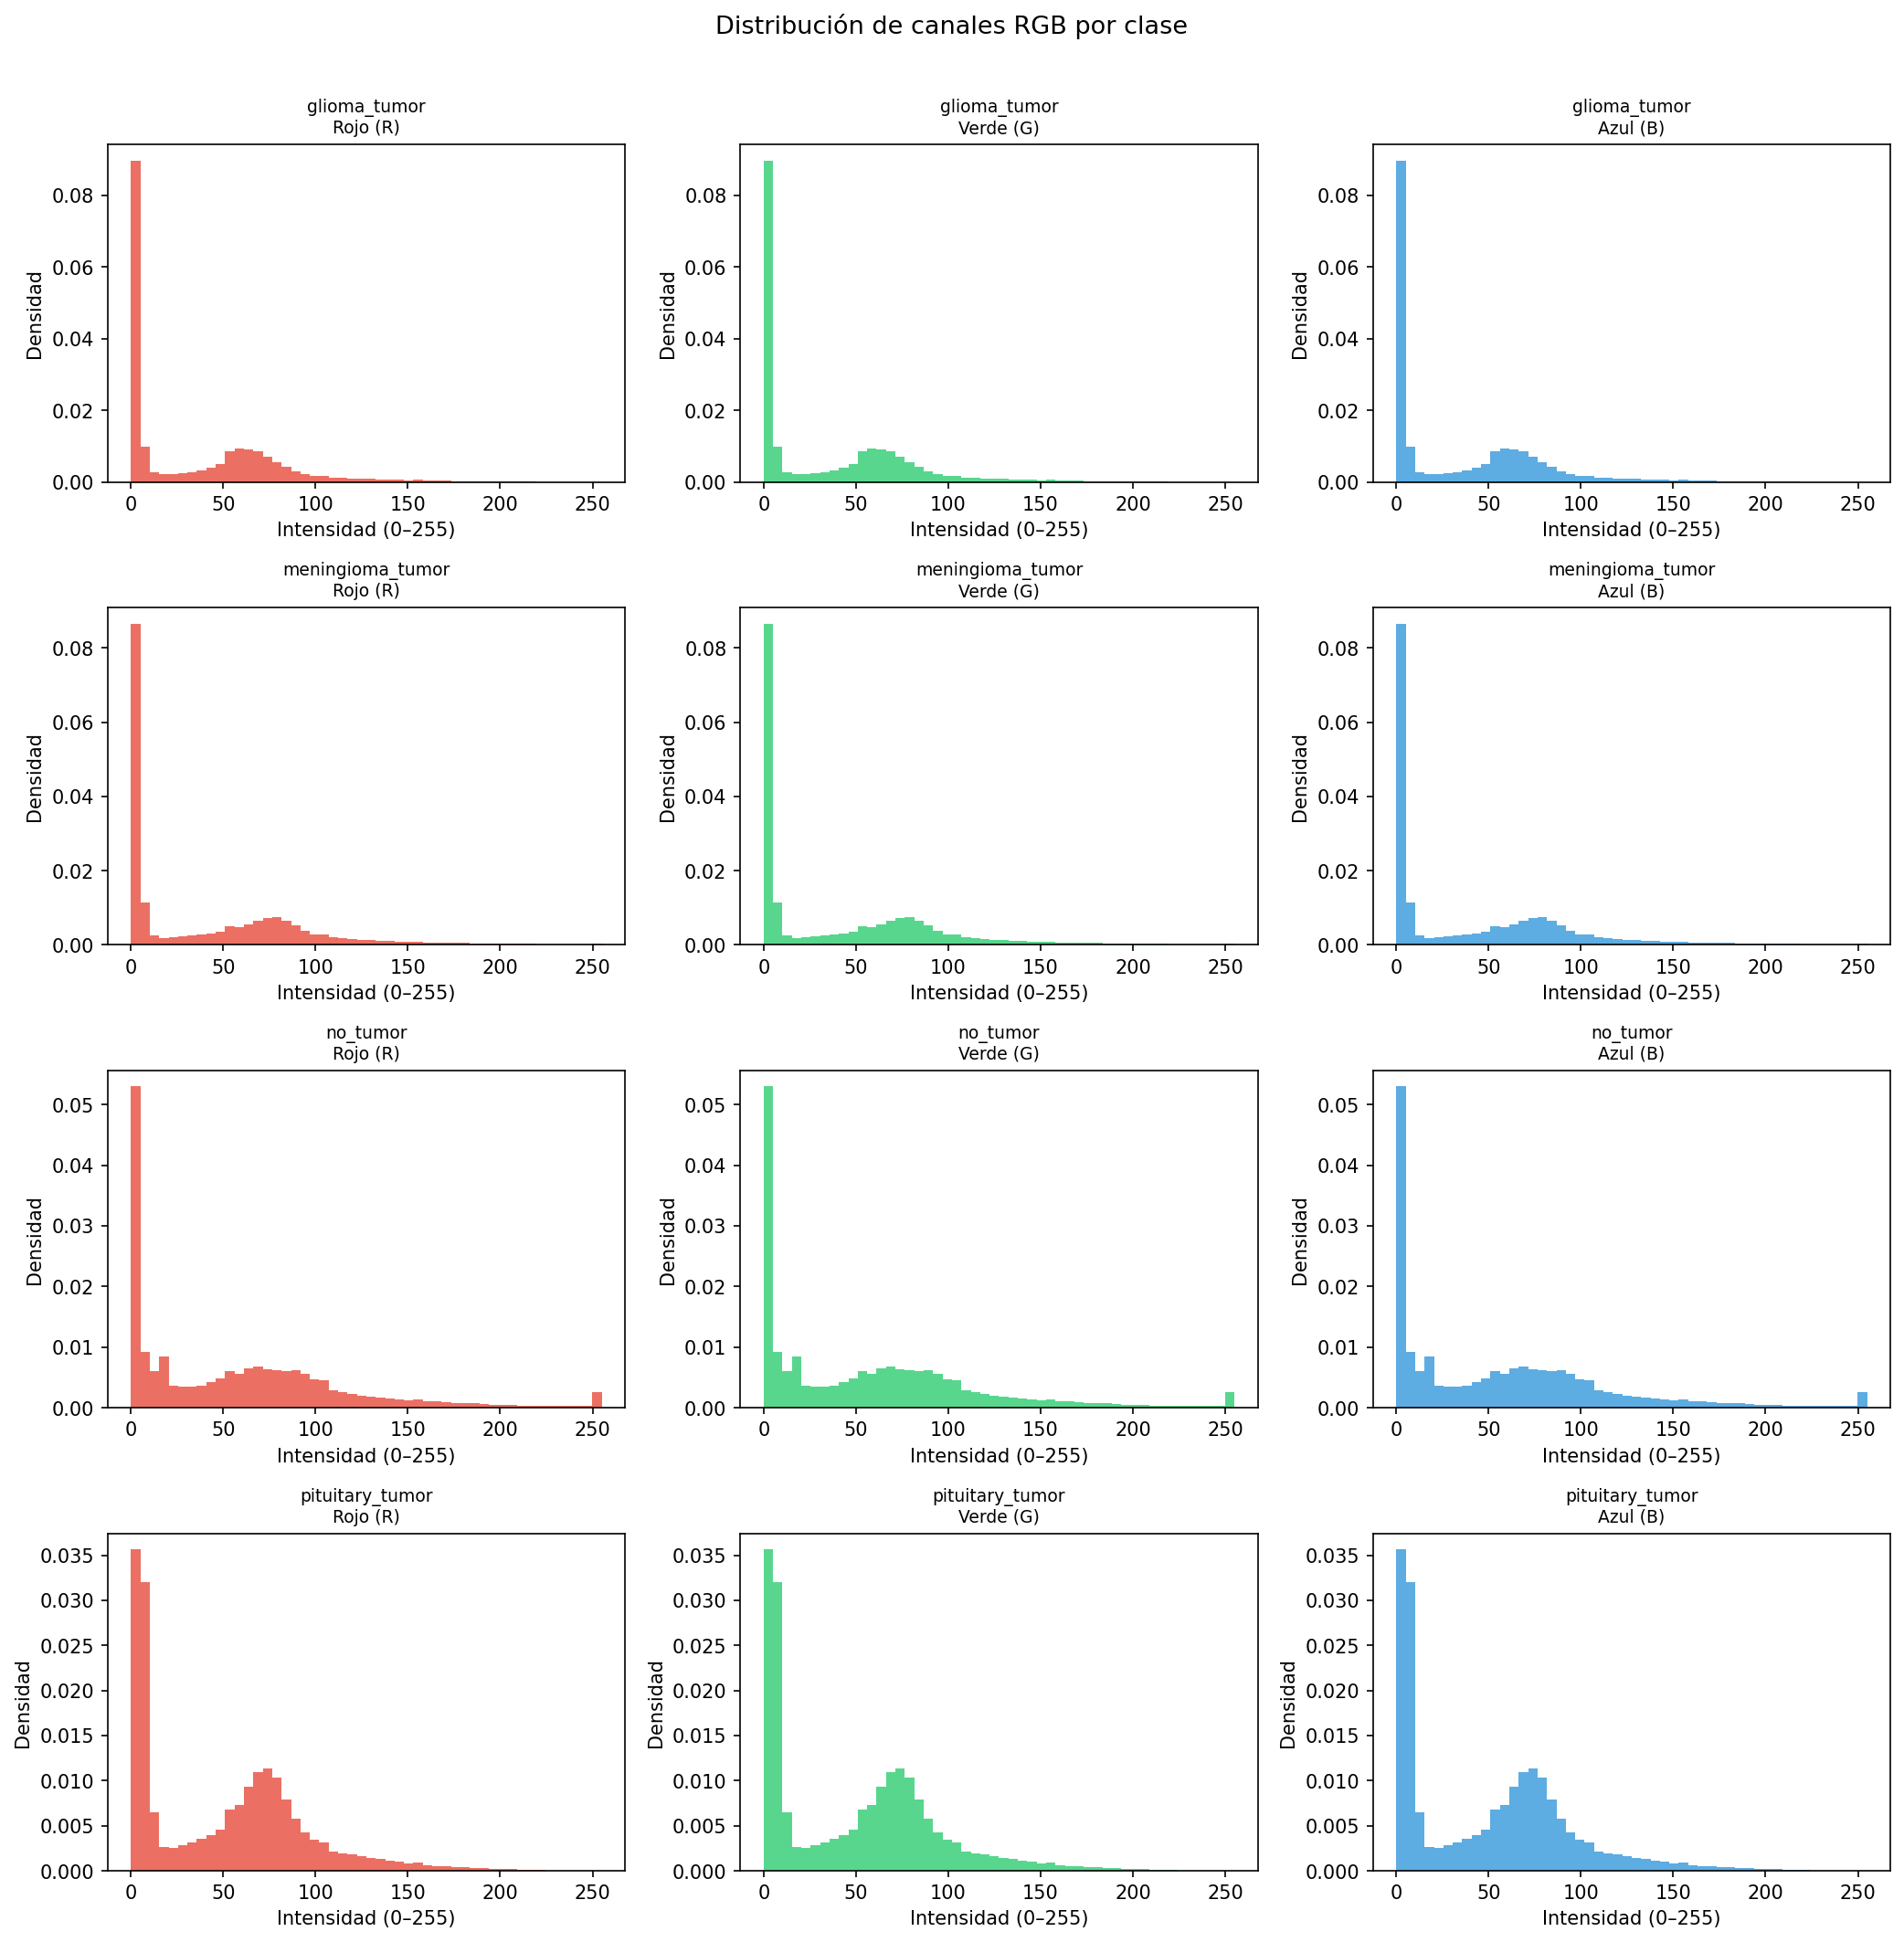
\includegraphics[width=\columnwidth]{../../outputs/figures/canales_rgb.png}
\caption{Distribución de intensidades por canal RGB y por
clase.}
\label{fig:rgb}
\end{figure}

\subsection{Imagen Promedio y Muestras por Clase}
La Figura~\ref{fig:promedio} presenta la imagen promedio por
clase, calculada como la media píxel a píxel de 100 imágenes
redimensionadas a 224$\times$224\,px. Los gliomas exhiben
regiones \textbf{hipointensas difusas}, de bordes poco
definidos, consistente con su naturaleza infiltrativa. Los
tumores \textit{pituitarios} tienden a concentrarse en la zona
central, reflejando la ubicación anatómica de la glándula
hipófisis. Los meningiomas muestran patrones intermedios con
tendencia a localizarse en la periferia. La clase
\textit{no\_tumor}, al promediar tejidos cerebrales sanos en
distintas orientaciones, produce una imagen más difusa y
centralmente simétrica.

\begin{figure}[!t]
\centering
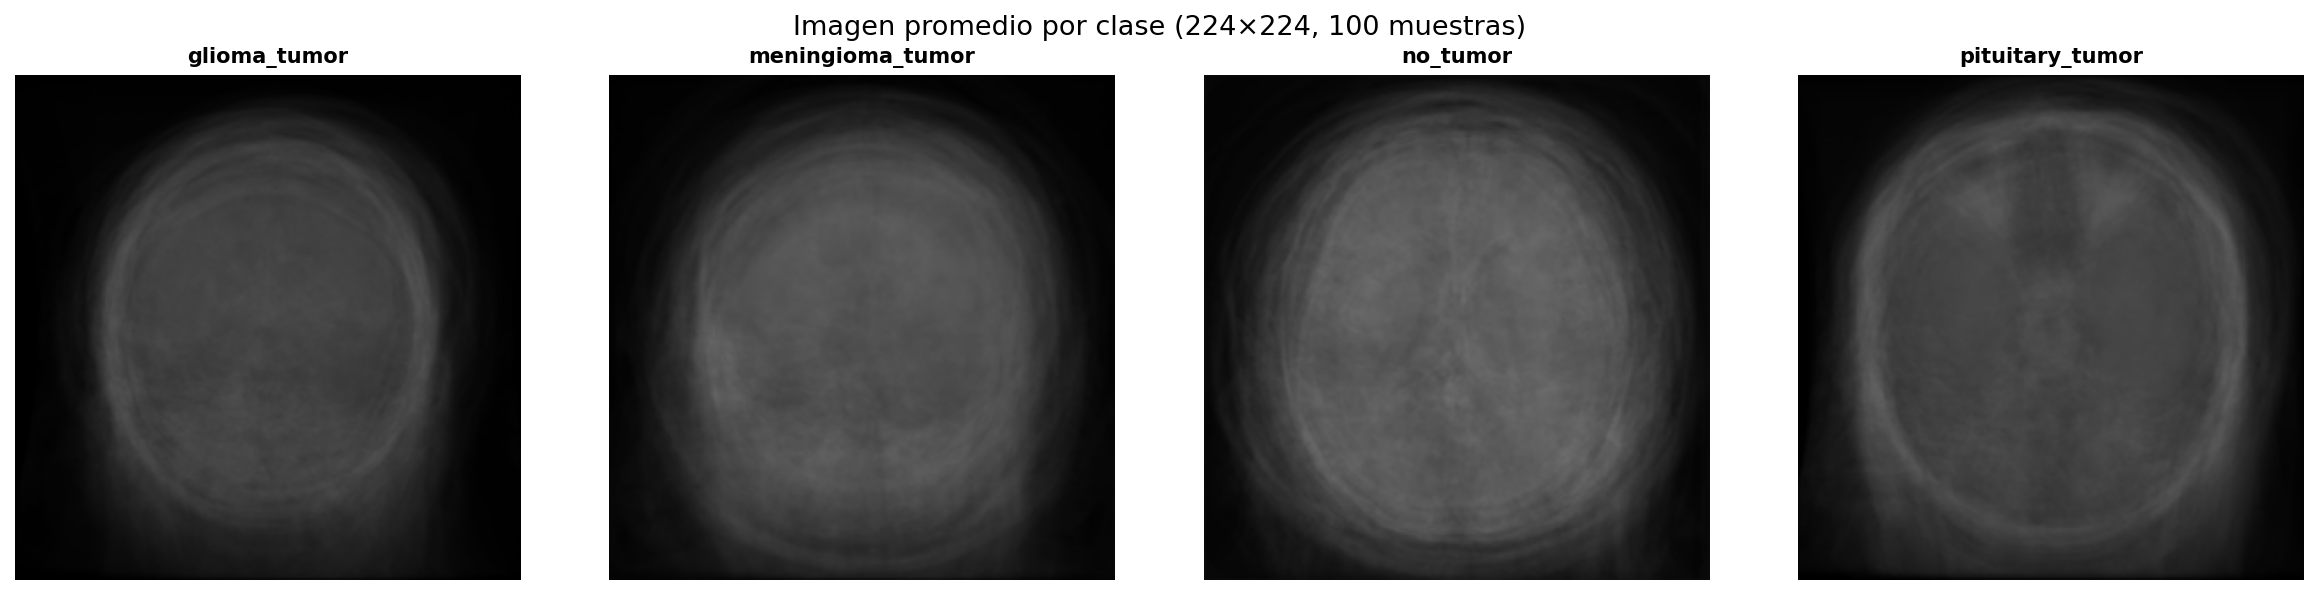
\includegraphics[width=\columnwidth]{../../outputs/figures/imagen_promedio.png}
\caption{Imagen promedio por clase (100 imgs, 224$\times$224
px).}
\label{fig:promedio}
\end{figure}

La Figura~\ref{fig:muestras} ilustra cinco ejemplos
representativos por clase. Se evidencia alta variabilidad
intra-clase en orientación, escala y contraste, lo que justifica
el uso de \textit{data augmentation} ---rotación
$\pm 15^{\circ}$, \textit{flip} horizontal y variación de
brillo--- durante el entrenamiento para mejorar la capacidad de
generalización del modelo.

\begin{figure}[!t]
\centering
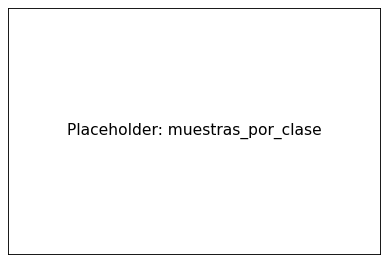
\includegraphics[width=\columnwidth]{../../outputs/figures/muestras_por_clase.png}
\caption{5 muestras por clase --- \textit{Training}.}
\label{fig:muestras}
\end{figure}

\subsection{Plan de Preprocesamiento}
A partir de los hallazgos anteriores, se define el pipeline de
preprocesamiento resumido en la Tabla~\ref{tab:pipe}, aplicado
de forma consistente a las tres arquitecturas evaluadas.

\begin{table}[!t]
\centering
\caption{Pipeline de preprocesamiento propuesto.}
\label{tab:pipe}
\begin{tabularx}{\columnwidth}{clX}
\toprule
\textbf{\#} & \textbf{Paso} & \textbf{Justificación} \\
\midrule
1 & Resize 224$\times$224\,px & Resoluciones heterogéneas requieren entrada uniforme. \\
2 & Conversión a RGB           & Algunas imágenes en escala de grises; se unifica formato. \\
3 & Z-score ($\mu$ ImageNet)   & Estabiliza el gradiente y mejora la convergencia. \\
4 & \textit{Data augmentation} & Rotación $\pm 15^{\circ}$, \textit{flip} horizontal y variación de brillo. \\
5 & \textit{class\_weight}     & Compensa el desbalance de \textit{no\_tumor}. \\
6 & Split 80/20 \textit{Training} & Separa validación sin contaminar el \textit{holdout} oficial. \\
\bottomrule
\end{tabularx}
\end{table}

\section{Metodología}

\subsection{Métricas de Evaluación}
Para evaluar las arquitecturas propuestas se emplea un conjunto
de métricas estándar de clasificación multiclase:

\begin{itemize}
  \item \textbf{Accuracy:} proporción global de aciertos,
        $\text{Acc} = (TP+TN)/(TP+TN+FP+FN)$.
  \item \textbf{Precision (macro):} promedio no ponderado de la
        precisión por clase,
        $\tfrac{1}{C}\sum_{c} TP_c/(TP_c+FP_c)$.
  \item \textbf{Recall (macro):} promedio no ponderado de la
        sensibilidad por clase,
        $\tfrac{1}{C}\sum_{c} TP_c/(TP_c+FN_c)$.
  \item \textbf{F1-Score (macro):} media armónica de Precision y
        Recall, $F1 = 2 \cdot P \cdot R / (P+R)$, calculada por
        clase y promediada de forma no ponderada.
  \item \textbf{Matriz de confusión:} análisis cualitativo de
        los errores entre pares de clases.
\end{itemize}

Dado el desbalance descrito en la Sección~\ref{sec:eda}, la
\textit{Accuracy} puede ser engañosa, pues un modelo que ignore
por completo la clase \textit{no\_tumor} aún alcanzaría valores
razonables. El \textbf{F1-Score macro} otorga el mismo peso a
todas las clases sin considerar su frecuencia, por lo que
penaliza explícitamente los modelos que descuidan las clases
minoritarias. Por esta razón se adopta como métrica principal
de comparación entre los tres modelos.

\subsection{Arquitectura Modelo 1 --- CNN Baseline}
\label{sec:arq-m1}

La arquitectura del Modelo~1 fue diseñada como un \textit{baseline}
convolucional ligero, inspirado en la red OkanNet propuesta por
Uçar y Kurt~\cite{okannet2026} y en la CNN desde cero de Gupta
\textit{et al.}~\cite{gupta2023}. Se compone de tres bloques
convolucionales secuenciales seguidos de un cabezal denso, sin
emplear \textit{Batch Normalization} ni conexiones residuales, de
modo que sirva como punto de referencia frente a los Modelos~2
y~3.

\begin{table}[!t]
\centering
\caption{Arquitectura del Modelo~1 (CNN Baseline). Entrada
$(B, 3, 224, 224)$.}
\label{tab:arq-m1}
\renewcommand{\arraystretch}{1.15}
\setlength{\tabcolsep}{4pt}
\footnotesize
\begin{tabular}{@{}clccccr@{}}
\toprule
\textbf{\#} & \textbf{Capa} & \textbf{Filt.} & \textbf{Kernel} &
\textbf{Stride} & \textbf{Salida $(C,H,W)$} & \textbf{Params} \\
\midrule
1  & Conv2D       & 16 & $3{\times}3$ & 1  & $(16,224,224)$ & $448$         \\
2  & ReLU         & -- & --           & -- & $(16,224,224)$ & $0$           \\
3  & MaxPool2D    & -- & $2{\times}2$ & 2  & $(16,112,112)$ & $0$           \\
4  & Conv2D       & 32 & $3{\times}3$ & 1  & $(32,112,112)$ & $4\,640$      \\
5  & ReLU         & -- & --           & -- & $(32,112,112)$ & $0$           \\
6  & MaxPool2D    & -- & $2{\times}2$ & 2  & $(32,56,56)$   & $0$           \\
7  & Conv2D       & 64 & $3{\times}3$ & 1  & $(64,56,56)$   & $18\,496$     \\
8  & ReLU         & -- & --           & -- & $(64,56,56)$   & $0$           \\
9  & MaxPool2D    & -- & $2{\times}2$ & 2  & $(64,28,28)$   & $0$           \\
10 & Flatten      & -- & --           & -- & $(50\,176,)$   & $0$           \\
11 & Linear       & -- & --           & -- & $(128,)$       & $6\,422\,656$ \\
12 & ReLU         & -- & --           & -- & $(128,)$       & $0$           \\
13 & Dropout(0.5) & -- & --           & -- & $(128,)$       & $0$           \\
14 & Linear       & -- & --           & -- & $(4,)$         & $516$         \\
\midrule
\multicolumn{6}{r}{\textbf{Total parámetros entrenables:}} & $\mathbf{6\,446\,756}$ \\
\bottomrule
\end{tabular}
\end{table}

Las decisiones de diseño se justifican como sigue:

\begin{itemize}
  \item \textbf{Tres bloques convolucionales} con filtros
        $16{\to}32{\to}64$, replicando la progresión geométrica
        de OkanNet~\cite{okannet2026}. Esta profundidad limitada
        deja margen explícito para que los Modelos~2 y~3
        muestren mejoras atribuibles a su mayor complejidad.
  \item \textbf{Kernels} $3{\times}3$ con \textit{padding}
        \textit{same} y \textbf{MaxPool} $2{\times}2$ con
        \textit{stride}~2: configuración estándar en la
        literatura de clasificación MRI~\cite{gupta2023} que
        preserva la información espacial dentro de cada bloque
        y la reduce a la mitad entre bloques.
  \item \textbf{Sin \textit{Batch Normalization}}: decisión
        deliberada del enunciado, para aislar el efecto que
        introducirá el Modelo~2 al añadir BN.
  \item \textbf{Cabezal denso}: \texttt{Linear(50\,176, 128)}
        $\to$ \texttt{ReLU} $\to$ \texttt{Dropout(0{,}5)} $\to$
        \texttt{Linear(128, 4)}. El \textit{Dropout} en la única
        capa oculta del cabezal sigue la práctica de
        OkanNet~\cite{okannet2026} y mitiga el sobreajuste sin
        introducir regularización adicional.
  \item \textbf{Inicialización}: \textit{Kaiming Normal} en las
        capas \texttt{Conv2D} (modo \texttt{fan\_out}) y en las
        capas \texttt{Linear} (modo \texttt{fan\_in}). Esta
        separación es crucial: una inicialización
        \texttt{fan\_out} aplicada a
        \texttt{Linear(50\,176, 128)} produciría una magnitud
        de preactivaciones tan elevada que rompería la
        convergencia, especialmente cuando se introduce BN.
\end{itemize}

El número total de parámetros entrenables es de $6\,446\,756$,
dominado casi en su totalidad ($\approx 99{,}6$\,\%) por la
primera capa totalmente conectada, lo cual es un patrón típico
de arquitecturas tipo LeNet/AlexNet sin
\textit{Global Average Pooling}.

\subsubsection*{Arquitectura comparativa OkanNet}

Como contraste académico se implementó una versión \emph{réplica}
de OkanNet~\cite{okannet2026}, idéntica al Modelo~1 pero con
\textit{Batch Normalization 2D} añadido entre cada \texttt{Conv2D}
y su \texttt{ReLU}. El total de parámetros asciende a
$6\,446\,980$ ($+224$ por las medias y varianzas aprendibles de
BN), y los hiperparámetros de entrenamiento se mantienen
idénticos al \textit{baseline} para que la única variable que
cambia entre ambas redes sea precisamente la presencia de BN.

\subsection{Arquitectura Modelo 2 --- CNN Profunda}
\textit{[PENDIENTE: descripción detallada del \texttt{model 2},
incluyendo el uso de \textit{Batch Normalization} entre las
capas convolucionales, \textit{Dropout} en las capas densas,
mayor profundidad (bloques convolucionales adicionales) y
justificación de cada elemento frente al \textit{baseline}.]}

\subsection{Arquitectura Modelo 3 --- CNN con Técnica Avanzada}
\textit{[PENDIENTE: descripción del \texttt{model 3}, integrando
una técnica avanzada construida desde cero (por ejemplo, bloques
residuales tipo ResNet, \textit{Global Average Pooling}, módulos
de atención o conexiones densas), manteniendo la restricción de
no usar pesos preentrenados.]}

\section{Entrenamiento e Implementación}

\subsection{Hiperparámetros}
\label{sec:hiperparam}

La Tabla~\ref{tab:hiperparam} resume los hiperparámetros
empleados para entrenar el Modelo~1 y su comparativa OkanNet.
Para garantizar una comparación científicamente limpia, se
mantienen idénticos en ambas arquitecturas; la única diferencia
controlada entre ellas es la presencia de
\textit{Batch Normalization}.

\begin{table}[!t]
\centering
\caption{Hiperparámetros del Modelo~1 (Baseline) y OkanNet.}
\label{tab:hiperparam}
\renewcommand{\arraystretch}{1.15}
\footnotesize
\begin{tabular}{@{}lll@{}}
\toprule
\textbf{Hiperparámetro} & \textbf{Baseline} & \textbf{OkanNet} \\
\midrule
Optimizador               & Adam                      & Adam                      \\
\quad $(\beta_1, \beta_2)$ & $(0{,}9, 0{,}999)$        & $(0{,}9, 0{,}999)$        \\
Learning rate inicial     & $1\times 10^{-3}$         & $1\times 10^{-3}$         \\
Scheduler                 & ReduceLROnPlateau         & ReduceLROnPlateau         \\
\quad factor / patience   & $0{,}5$ / $3$             & $0{,}5$ / $3$             \\
\quad $\eta_{\min}$       & $1\times 10^{-6}$         & $1\times 10^{-6}$         \\
Función de pérdida        & \texttt{CrossEntropyLoss} & \texttt{CrossEntropyLoss} \\
\quad con                 & \texttt{class\_weight}    & \texttt{class\_weight}    \\
\textit{Weight decay}     & $0$                       & $0$                       \\
\textit{Batch size}       & $32$                      & $32$                      \\
\textit{Epochs} máx.      & $40$                      & $40$                      \\
\textit{Early stopping}   & patience $=7$             & patience $=7$             \\
\quad criterio            & F1-macro val.             & F1-macro val.             \\
\textit{Split} train/val  & 80\,\%\,/\,20\,\%          & 80\,\%\,/\,20\,\%          \\
\textit{Seed}             & $42$                      & $42$                      \\
\bottomrule
\end{tabular}
\end{table}

El uso de \texttt{class\_weight} en la función de pérdida es un
diferencial del presente trabajo frente a las referencias
revisadas~\cite{okannet2026,gupta2023}, ninguna de las cuales
incorpora corrección explícita del desbalance de clases. Los
pesos se calculan con la fórmula \textit{balanced} de
\texttt{scikit-learn}, inversamente proporcionales a la
frecuencia de cada clase en \textit{Training}.

El tiempo de entrenamiento sobre Apple Silicon con backend MPS
fue de $7$\,min $44$\,s para el Baseline y $3$\,min $39$\,s
para OkanNet, este último interrumpido por \textit{early
stopping} en la época~$17$.

\subsubsection*{Hiperparámetros del Modelo~2}
\label{sec:hiperparam-m2}

Las dos variantes del Modelo~2 (DeepCNN-BN y DeepCNN-BN-GAP)
comparten un régimen de entrenamiento propio, distinto al del
Modelo~1, motivado por el fallo de OkanNet:

\begin{table*}[!t]
\centering
\caption{Hiperparámetros del Modelo~2 (DeepCNN-BN y
DeepCNN-BN-GAP). Idénticos en ambas variantes para aislar el
efecto del cabezal.}
\label{tab:hiperparam-m2}
\renewcommand{\arraystretch}{1.15}
\footnotesize
\begin{tabular}{@{}lll@{}}
\toprule
\textbf{Hiperparámetro} & \textbf{Modelo 2} & \textbf{vs Modelo 1} \\
\midrule
Optimizador               & AdamW                     & Adam                    \\
\quad $(\beta_1, \beta_2)$ & $(0{,}9, 0{,}999)$        & idéntico                \\
\textit{Learning rate}    & $5\times 10^{-4}$         & $10^{-3}$ (M1)          \\
\textit{Weight decay}     & $10^{-4}$                 & $0$                     \\
\textit{Batch size}       & $64$                      & $32$ (M1)               \\
Scheduler                 & ReduceLROnPlateau         & idéntico                \\
\quad factor / patience   & $0{,}5$ / $3$             & idéntico                \\
\quad $\eta_{\min}$       & $10^{-6}$                 & idéntico                \\
Función de pérdida        & \texttt{CrossEntropyLoss} & idéntico                \\
\quad con                 & \texttt{class\_weight}    & idéntico                \\
\textit{Epochs} máx.      & $50$                      & $40$ (M1)               \\
\textit{Early stopping}   & patience $=8$             & patience $=7$ (M1)      \\
\quad criterio            & F1-macro val.             & idéntico                \\
\textit{Split} train/val  & 80\,\%\,/\,20\,\%         & idéntico                \\
\textit{Seed}             & $42$                      & idéntico                \\
\bottomrule
\end{tabular}
\end{table*}

Tres ajustes distinguen al Modelo~2 del Modelo~1:

\begin{enumerate}
  \item \textbf{Optimizador AdamW en lugar de Adam.} La
        diferencia clave es que AdamW desacopla
        \textit{weight decay} del gradiente, evitando el
        sesgo que Adam clásico introduce al combinar
        \textit{L2 regularization} con momento
        adaptativo~\cite{loshchilov2017decoupled}. Esto
        habilita el uso de \textit{weight decay} no nulo
        ($10^{-4}$) como regularización adicional.
  \item \textbf{\textit{Learning rate} reducido y
        \textit{batch size} duplicado.} La combinación
        $\text{lr}=10^{-3}$ con $\text{batch}=32$
        empleada en el Modelo~1 generó inestabilidad en
        OkanNet (véase Tabla~\ref{tab:metricas-global}). En el
        Modelo~2 se baja \textit{lr} a $5\times 10^{-4}$ y se
        sube \textit{batch size} a $64$ para reducir la
        varianza de las estadísticas estimadas por
        \textit{mini-batch} en BN: con $\text{batch}=64$ la
        estimación de medias y varianzas es más estable, lo
        que evita el ``ruido amplificado'' que en OkanNet
        provocó la divergencia.
  \item \textbf{Mayor horizonte de entrenamiento.} El número
        máximo de épocas sube de $40$ a $50$ y la paciencia
        de \textit{early stopping} de $7$ a $8$, pues el
        \textit{backbone} más profundo requiere más
        iteraciones para converger.
\end{enumerate}

Bajo este régimen, ambas variantes se entrenan con los mismos
hiperparámetros para que la única variable que distingue a
DeepCNN-BN de DeepCNN-BN-GAP sea, efectivamente, el cabezal
(FC vs GAP).

\subsection{Protocolo de Entrenamiento}
\label{sec:proto}
La implementación se realiza íntegramente en \textbf{Python} con
\textbf{PyTorch}, mediante \textit{scripts} locales organizados
en el directorio \texttt{src/}. El flujo de trabajo reproducible
es el siguiente:

\begin{enumerate}
  \item Crear un entorno virtual aislado:
        \texttt{python -m venv .venv} y activarlo.
  \item Instalar dependencias:
        \texttt{pip install -r requirements.txt}.
  \item Lanzar el entrenamiento de un modelo específico:\\
        \texttt{python src/models/train.py -{}-model N\\
        -{}-data\_dir datasets/Training},
        con \texttt{N} $\in \{1, 2, 3\}$.
  \item Los \textit{checkpoints} de pesos se almacenan en
        \texttt{outputs/results/} y las métricas por época se
        registran incrementalmente en
        \texttt{outputs/results/metrics.csv}.
  \item La evaluación final sobre el conjunto de prueba se
        ejecuta con:\\
        \texttt{python src/models/evaluate.py -{}-model N\\
        -{}-data\_dir datasets/Testing}.
\end{enumerate}

Se aplica una división interna \textbf{80/20} sobre el conjunto
\textit{Training} para obtener un \textit{validation set} usado
en la monitorización de pérdida y métricas durante el
entrenamiento y en la selección del mejor \textit{checkpoint}.
El conjunto \textit{Testing} original se reserva como
\textit{holdout} independiente y solo se emplea en la evaluación
final reportada en la sección de resultados.

\subsection{Hiperparámetros Modelo 3}
\label{sec:hiperparam-m3}

La Tabla~\ref{tab:hiperparam-m3} resume los hiperparámetros
empleados para entrenar el Modelo~3 (MRIResNet).
Las diferencias más relevantes respecto al Modelo~1 son el uso
de \textbf{AdamW} con \textit{weight decay} desacoplado ---en
lugar de Adam sin regularización--- y un \textit{learning rate}
inicial diez veces menor, coherente con la mayor profundidad de la
red y la presencia de \textit{Batch Normalization} en todos los
bloques residuales.

\begin{table}[!t]
\centering
\caption{Hiperparámetros del Modelo~3 (MRIResNet).}
\label{tab:hiperparam-m3}
\renewcommand{\arraystretch}{1.15}
\footnotesize
\begin{tabular}{@{}ll@{}}
\toprule
\textbf{Hiperparámetro} & \textbf{MRIResNet (M3)} \\
\midrule
Optimizador                 & AdamW                     \\
\quad $(\beta_1, \beta_2)$  & $(0{,}9,\;0{,}999)$       \\
Learning rate inicial       & $1\times10^{-4}$          \\
\textit{Weight decay}       & $1\times10^{-4}$          \\
Scheduler                   & ReduceLROnPlateau         \\
\quad factor / patience     & $0{,}5$ / $5$             \\
\quad $\eta_{\min}$         & $1\times10^{-6}$          \\
Función de pérdida          & CrossEntropyLoss          \\
\quad con                   & \texttt{class\_weight}    \\
\textit{Batch size}         & $32$                      \\
\textit{Epochs} máx.        & $50$                      \\
\textit{Early stopping}     & patience $= 10$           \\
\quad criterio              & F1-macro val.             \\
\textit{Split} train/val  & 80\% / 20\% \\
\textit{Seed}               & $42$                      \\
\midrule
Canales de entrada          & $5$ (R, G, B, CLAHE, Sobel) \\
Parámetros entrenables      & $1\,676\,284$             \\
\bottomrule
\end{tabular}
\end{table}

La elección de \textbf{AdamW} frente a Adam responde a que el
\textit{weight decay} desacoplado de AdamW actúa como
regularización $L_2$ explícita independiente del \textit{learning
rate}, lo cual es especialmente beneficioso en redes con
\textit{Batch Normalization}~\cite{loshchilov2019adamw}.
El uso de \texttt{class\_weight} calculado con la fórmula
\textit{balanced} de \texttt{scikit-learn} se mantiene respecto
al Modelo~1 para corregir el desbalance documentado en la
Sección~\ref{sec:hiperparam}.

El protocolo de entrenamiento es análogo al descrito en la
Sección~\ref{sec:proto}: división 80/20, monitorización del
F1-macro de validación para el \textit{scheduler} y el
\textit{early stopping}, y registro de métricas por época en
un archivo \texttt{.csv}.

\section{Resultados}

\subsection{Métricas por Modelo}
\textit{[PENDIENTE: incluir tabla comparativa con Accuracy,
Precision (macro), Recall (macro) y F1-Score (macro) obtenidos
sobre el conjunto de prueba para \texttt{model 1},
\texttt{model 2} y \texttt{model 3}.]}

\subsection{Análisis por Clase}
\textit{[PENDIENTE: tabla con F1-Score por clase para cada
modelo, destacando las clases con menor desempeño. Se anticipa
que \textit{meningioma\_tumor} podría ser la clase más difícil
debido a la similitud visual de sus patrones con otras lesiones
intracraneales.]}

\subsection{Matrices de Confusión}
\textit{[PENDIENTE: inserción de
\texttt{\textbackslash includegraphics} con las matrices de
confusión generadas en \texttt{confusion\_modelN.png} para los
tres modelos, con análisis cualitativo de los principales
patrones de error.]}

\subsection{Curvas de Entrenamiento}
\textit{[PENDIENTE: curvas de \textit{loss} y \textit{accuracy}
(train vs.\ val) por época para cada modelo, generadas desde
\texttt{outputs/results/metrics.csv}, con análisis de
convergencia, presencia de \textit{overfitting} y efectividad
del \textit{scheduler}.]}

\section{Conclusiones}
\label{sec:conclusiones}

\textit{[PENDIENTE: discusión final estructurada en cuatro ejes:
(i) si los resultados obtenidos por las CNN propias permiten
considerar el sistema como una herramienta de apoyo diagnóstico
clínicamente confiable; (ii) análisis de las clases problemáticas
y sus posibles causas (similitud fotométrica, desbalance,
variabilidad intra-clase); (iii) limitaciones del enfoque sin
\textit{transfer learning} y comparación cualitativa con
literatura que sí lo emplea; y (iv) trabajo futuro, incluyendo
\textit{transfer learning} desde redes preentrenadas,
segmentación previa de la región de interés, ampliación del
dataset y validación con datos clínicos externos.]}

\subsection*{Hallazgos del Modelo 2}

El Modelo~2 (DeepCNN-BN y DeepCNN-BN-GAP) permite cerrar tres
preguntas planteadas a la luz de los resultados del Modelo~1:

\begin{enumerate}
  \item \textbf{¿Es \textit{Batch Normalization} responsable
        del colapso de OkanNet?} \textbf{No.} Bajo el régimen
        adaptado (AdamW, lr=$5\times 10^{-4}$, bs=$64$,
        wd=$10^{-4}$), una red con $10$ capas convolucionales
        y BN tras cada una alcanza F1-macro de $0{,}5961$ en
        \textit{Testing} ---$+17{,}28$ puntos porcentuales
        sobre OkanNet---, con curvas de convergencia
        monótonas y sin oscilaciones. El colapso de OkanNet
        era atribuible a la combinación lr=$10^{-3}$ /
        bs=$32$, no a BN como técnica. La hipótesis sostenida
        en la Sección~\ref{sec:metricas-modelo} sobre el
        Modelo~1 queda confirmada.

  \item \textbf{¿Aporta el cabezal FC capacidad
        discriminativa real frente a GAP?} \textbf{Sí, en
        este dataset.} La variante DeepCNN-BN supera a
        DeepCNN-BN-GAP por $7{,}85$ puntos de F1-macro en
        \textit{Testing} ($0{,}5961$ vs $0{,}5176$), pese a
        compartir el \textit{backbone} convolucional. La
        brecha se concentra en las clases con mayor
        variabilidad intra-clase (\textit{meningioma\_tumor}:
        $+14{,}6$ pp). La hipótesis de que GAP rinde
        equivalentemente cuando el \textit{backbone} es
        suficientemente profundo \emph{no se sostiene} en
        este corpus: los $\sim 524$\,K parámetros adicionales
        del cabezal FC sí se traducen en mejor generalización.

  \item \textbf{¿Resuelve el aumento de capacidad el sesgo
        \textit{glioma}~$\to$~\textit{meningioma}?}
        \textbf{No.} El Modelo~2 reproduce, e incluso
        intensifica, el patrón Precision-Recall observado en
        el baseline: alta Precision ($1{,}0000$ en DeepCNN-BN)
        y bajísimo Recall ($0{,}1600$) sobre
        \textit{glioma\_tumor}. Esto descarta una explicación
        puramente arquitectónica del problema y refuerza la
        hipótesis de divergencia distribucional entre los
        \textit{splits} oficiales del dataset Sartaj Bhuvaji:
        los gliomas del \textit{Testing} parecen provenir de
        subtipos o protocolos de adquisición sub-representados
        en \textit{Training}, lo cual el modelo no puede
        compensar sin intervención en los datos.
\end{enumerate}

Como corolario práctico, el Modelo~2 \textbf{no supera al
baseline en \textit{Testing}} ($0{,}5961$ vs $0{,}6252$,
$-2{,}91$ pp), pese a triplicar la profundidad convolucional y
añadir múltiples capas de regularización. Esta caída,
consistente con la pérdida de $\sim 30$ puntos entre validación
y prueba que afecta a todas las arquitecturas evaluadas en
este trabajo, indica que el factor dominante de generalización
\textbf{no es la capacidad del modelo sino el \textit{distribution
shift} entre particiones}. Direcciones esperables para el
Modelo~3 incluyen estrategias específicamente orientadas a este
problema, como \textit{transfer learning} desde redes
preentrenadas (que ya capturan invariancias robustas frente al
\textit{shift}), aumento de datos basado en transformaciones
físicamente plausibles para MRI, o esquemas de
\textit{domain adaptation} entre \textit{splits}.


% ── Referencias ───────────────────────────────────────────────────
% \bibliographystyle{IEEEtran}
% \bibliography{referencias}

\end{document}
